\chapter{Evaluation}
\label{chap:c5}

In this chapter evaluation of proposed algorithms on two different graph processing frameworks is elaborated. Firstly we evaluate the properties and performance of the algorithms for subgraph isomorphism on PowerGraph. Secondly we show the heterogeneity of the communication costs for vertex synchronization in the problems of both subgraph isomorphism and geospatial simulation. At the end we use these algorithms to show GrapH outperforms PowerGraph with respect to communication.

The experiments were conducted on a cluster of 11 machines, each of which has 3.0GHz Intel Xeon CPU E5472 with 8 cores, and 32GB RAM. The machines are connected with 1 Gbps Ethernet.

\section{Evaluation of DSI and its variants on PowerGraph}

To evaluate the algorithms for subgraph isomorphism, we use the real-life datasets\footnote{http://snap.stanford.edu/data/index.html}: (a) Wiki-Vote records Wikipedia who-votes-on-whom network, which is a directed graph with 7,115 nodes and 103,689 directed edges. (b) ego-Twitter records social circles from Twitter, which is a directed graph with 81,306 nodes and 2,420,744 directed edges. In the experiments of this section, vertices are randomly assigned with a label from a label set of 5 distinct elements.

\subsection{Impact of Pattern Size}

The experiments are started with a random pattern and proceeded by adding vertices one by one and adding edges between the vertices. The size of the pattern varies from 2 vertices to 5 vertices. Our cluster is not able to execute when the pattern size reaches 6, as all the memories are exhausted. The data graph is Wiki-Vote, and the number of machines is 11. For optimized DSI and PDSI, the initial vertex is randomly chosen. For PDSI, the parameter proportion is 0.3. 

We evaluate the runtime and message amount of these three algorithms with different pattern sizes. Figure~\ref{fig:runtime-P} shows that the runtime of DSI and optimized DSI increases drastically as the pattern size grows, as the computational complexity is exponential to the pattern size. With two optimization strategies, the optimized DSI only takes about one third runtime as DSI needs. The runtime of PDSI does not increase so much as the boost of messages is limited by the proportion.

\begin{figure}[H]
  \begin{center}
    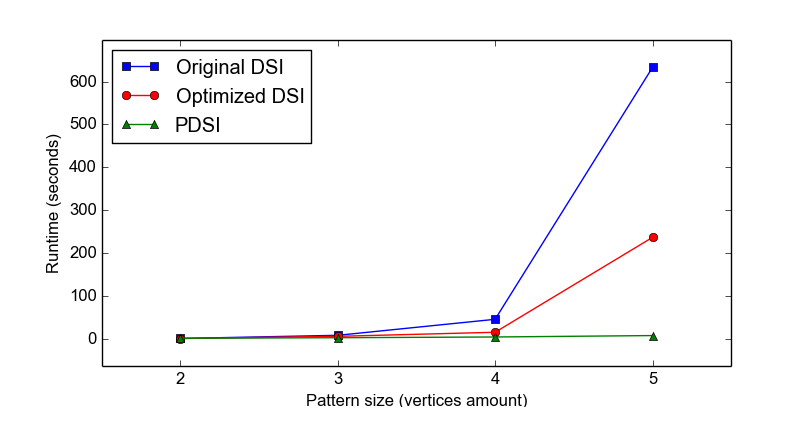
\includegraphics[width=\textwidth]{runtime-P.png}
    \caption{Runtime of DSI, optimized DSI and PDSI with patterns of different sizes}
    \label{fig:runtime-P}
  \end{center}
\end{figure}

Figure~\ref{fig:messages-P} shows that total message amount generated during the execution. The message amount is exponential to the pattern size. The runtime increases with same rate as the message amount grows, as the runtime mainly depends on how many messages to be processed.

\begin{figure}[H]
  \begin{center}
    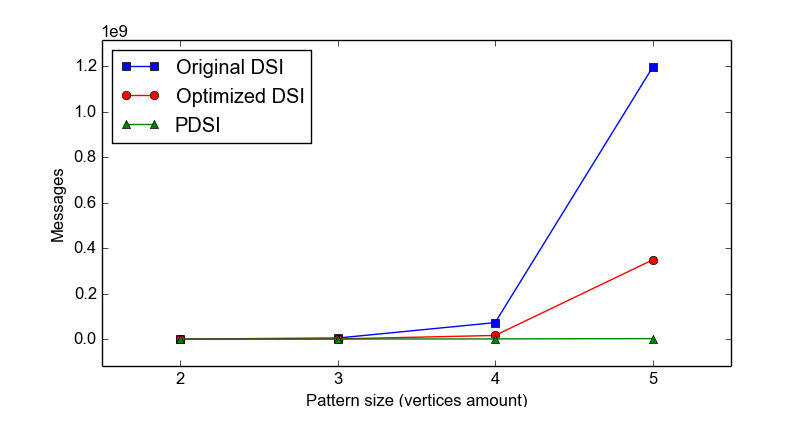
\includegraphics[width=\textwidth]{messages-Ps.png}
    \caption{Total message amount of DSI, optimized DSI and PDSI with patterns of different sizes}
    \label{fig:messages-P}
  \end{center}
\end{figure}

Another property of the algorithms to evaluate is the maximum supersteps. Table~\ref{tab:iterations} shows the how many supersteps that each algorithm has executed for different pattern sizes. All of them have the same amount of supersteps as the theoretical upper bound, which is $2 + k*(k-1)/2$ (our implementation uses one additional superstep to gather the neighboring vertices IDs). As the patterns are small and simple, it is possible to traverse the longest route in the data graph.

\newcolumntype{C}{>{\centering\arraybackslash}p{5em}}
\begin{table}[H]
  \begin{center}
    \begin{tabular}{|C|C|C|C|C|}
    \hline
    Pattern Size & DSI & Optimized DSI & PDSI & Upper Bound \\ \hline 
    2 & 3 & 3 & 3 & 3 \\ \hline
    3 & 5 & 5 & 5 & 5 \\ \hline
    4 & 8 & 8 & 8 & 8 \\ \hline
    5 & 12 & 12 & 12 & 12 \\ \hline
    \end{tabular}
    \caption{Supersteps of DSI, optimized DSI and PDSI with patterns of different sizes}
    \label{tab:iterations}
  \end{center}
\end{table}

We also evaluate the duplication of the found subgraphs. Figure~\ref{fig:repetitions-P} shows that subgraph duplication factor of the algorithms, which is the result that total found subgraphs amount is divided by the number of identical subgraphs. The duplication factor increases intensively as the pattern size grows. While DSI and optimized DSI have found the same number of identical subgraphs, DSI duplicates about 6000 times and optimized DSI duplicates about 1600 times when the pattern size is 5. It is mainly because the routes to find isomorphic subgraphs become more variant when the pattern size grows. PDSI does not guarantee that all subgraphs are found, but the duplication factor is relatively low.

\begin{figure}[H]
  \begin{center}
    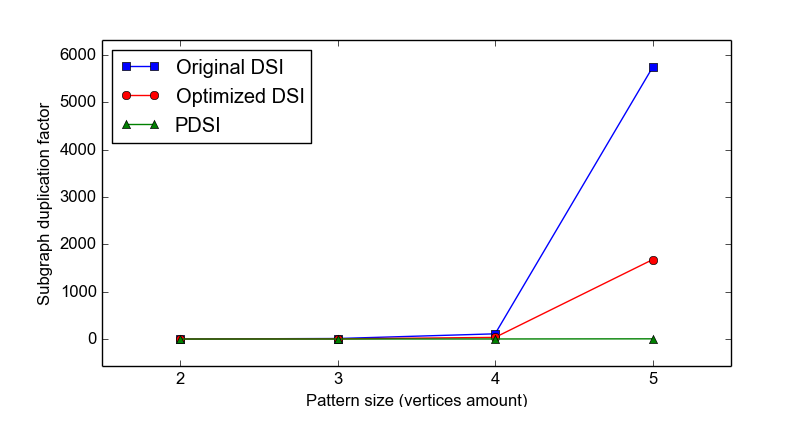
\includegraphics[width=\textwidth]{repetitions-Ps.png}
    \caption{Subgraph duplication factor of DSI, optimized DSI and PDSI with patterns of different sizes}
    \label{fig:repetitions-P}
  \end{center}
\end{figure}

As PDSI does not guarantee neither the existence nor the completeness of isomorphic subgraphs, we are interested in how many isomorphic subgraphs can be found by PDSI. Figure~\ref{fig:foundproportion-P} shows the percentage of the found identical subgraphs by PDSI. With the proportion 0.3, PDSI can find a large part of identical subgraphs, and has very low runtime and subgraph duplication factor.

\begin{figure}[H]
  \begin{center}
    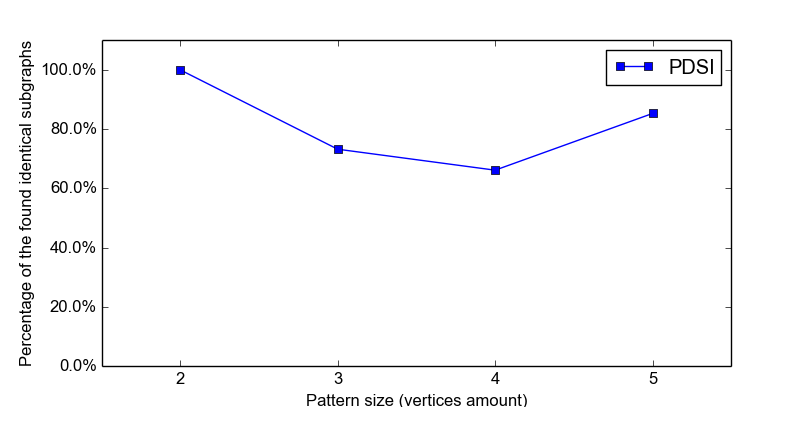
\includegraphics[width=\textwidth]{foundproportion-Ps.png}
    \caption{Percentage of the found identical subgraphs by PDSI with patterns of different sizes}
    \label{fig:foundproportion-P}
  \end{center}
\end{figure}

\subsection{Impact of Data Graph Size}

We evaluate the original DSI, optimized DSI and PDSI with data graphs of different sizes to study the properties of the algorithms. The data graphs we used are the subsets of ego-Twitter. The data graphs are increased by randomly adding vertices and their associating edges, which size varies from 42771 vertices to 81306 vertices. The pattern size is 3, and the number of machines is 11. For optimized DSI and PDSI, the initial vertex is randomly chosen. For PDSI, the parameter proportion is 0.1.

Figure~\ref{fig:runtime-G} shows that the runtime increases nonlinearly as the size of the data graph grows. The runtime behaviour also shows the computational complexity of the algorithms. The optimized DSI reduces the complexity and only takes about one third runtime as DSI needs. As PDSI uses the proportion to reduce the complexity, which also introduces non-deterministic factor to the runtime. Figure~\ref{fig:messages-G} shows that total message amount generated during the execution. The runtime increases with the same rate as the message amount grows.

\begin{figure}[H]
  \begin{center}
    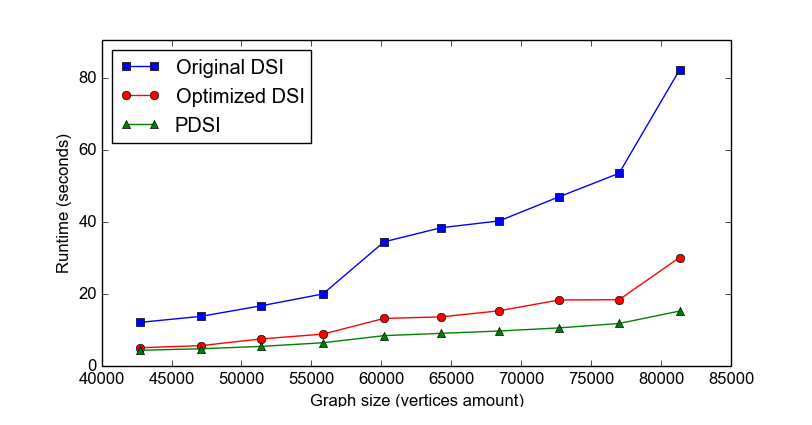
\includegraphics[width=\textwidth]{runtime-G.png}
    \caption{Runtime of DSI, optimized DSI and PDSI with data graphs of different sizes}
    \label{fig:runtime-G}
  \end{center}
\end{figure}

\begin{figure}[H]
  \begin{center}
    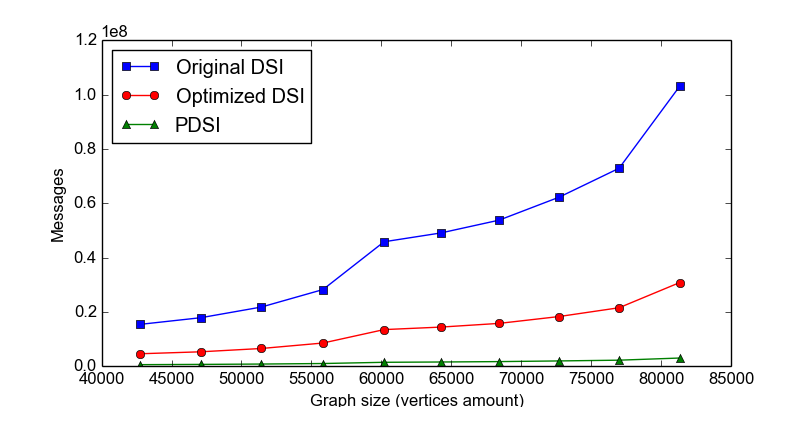
\includegraphics[width=\textwidth]{messages-Gs.png}
    \caption{Total message amount of DSI, optimized DSI and PDSI with data graphs of different sizes}
    \label{fig:messages-G}
  \end{center}
\end{figure}

\subsection{Impact of Machines}

We evaluate the runtime of original DSI, optimized DSI and PDSI with different number of machines to study the performance and scalability. The number of machines is increased from 2 to 11. The data graph is ego-Twitter and the pattern size is 3. For optimized DSI and PDSI, the initial vertex is randomly chosen. For PDSI, the parameter proportion is 0.1.

We can observe in Figure~\ref{fig:runtime-M} that PowerGraph scales very well with the three algorithms for subgraph isomorphism. With two optimization strategies, the optimized DSI only takes about one third runtime as DSI needs. PDSI with proportion 0.1 takes two third runtime as optimized DSI takes. The main reason is that execution with a pattern of size 3 do not have so many iterations. In addition, randomly selecting a proportion of messages in the gather phase introduces latency.

\begin{figure}[H]
  \begin{center}
    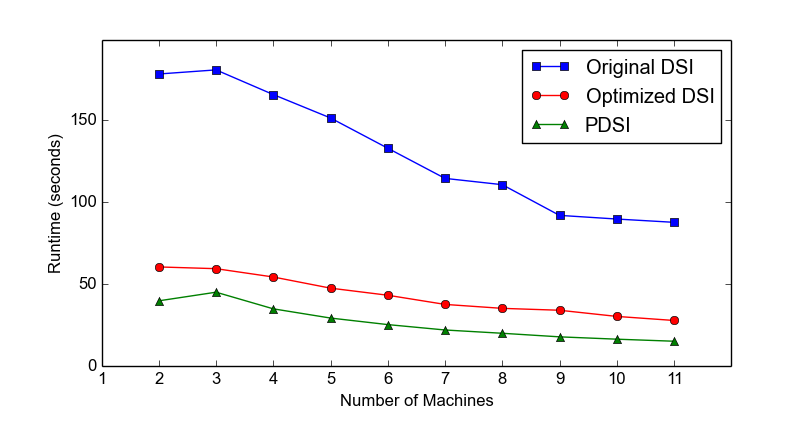
\includegraphics[width=\textwidth]{runtime-M.png}
    \caption{Runtime of DSI, optimized DSI and PDSI with different numbers of machines}
    \label{fig:runtime-M}
  \end{center}
\end{figure}

\subsection{Impact of the Proportion in PDSI}

The experiments were conducted by increasing the parameter proportion from 0.1 to 1. The data graph is ego-Twitter, the pattern size is 3, and the number of machines is 11. The initial vertex is randomly chosen. In Figure~\ref{fig:runtime-PP} we can see that the runtime can be well controlled by adopting different proportions. The runtime is almost linear to the proportion.

\begin{figure}[H]
  \begin{center}
    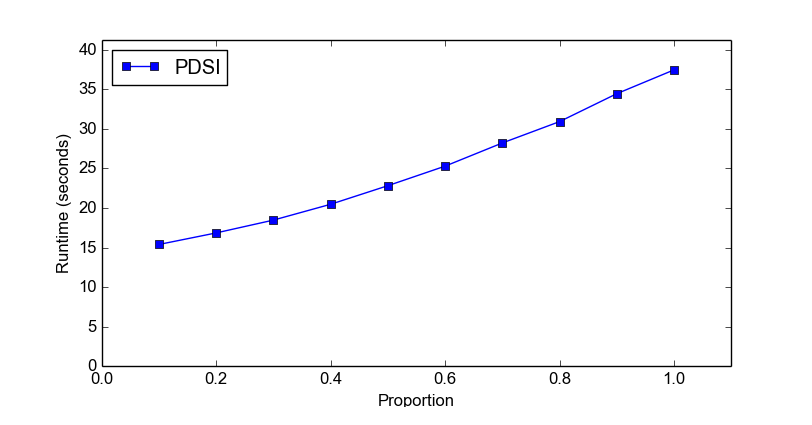
\includegraphics[width=\textwidth]{runtime-PP.png}
    \caption{Runtime of PDSI with different proportions}
    \label{fig:runtime-PP}
  \end{center}
\end{figure}

We show the duplication factor of PDSI with different proportions in Figure~\ref{fig:repetitions-PP}. The duplication factor increases with the proportion. High proportion leads to high messages quantity followed by high duplication factor.

\begin{figure}[H]
  \begin{center}
    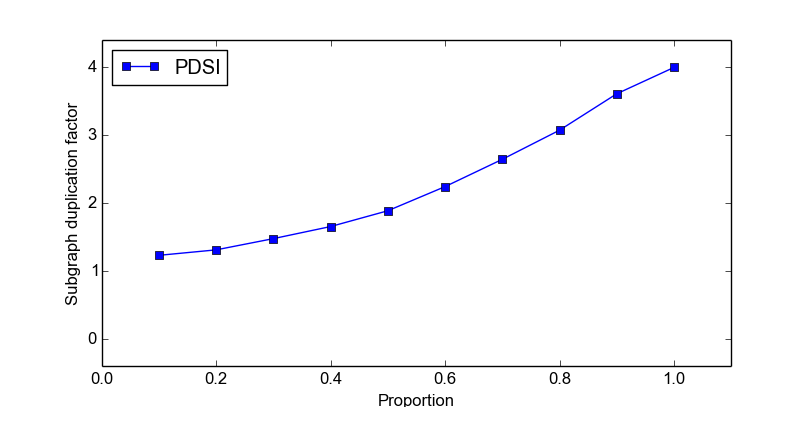
\includegraphics[width=\textwidth]{repetitions-PPs.png}
    \caption{Subgraph duplication factor of PDSI with different proportions}
    \label{fig:repetitions-PP}
  \end{center}
\end{figure}

Figure~\ref{fig:foundproportion-PP} shows that the percentage of found identical subgraphs increases with the proportion. We can see that PDSI can find more than 80\% of the subgraphs just with the proportion 0.5.

\begin{figure}[H]
  \begin{center}
    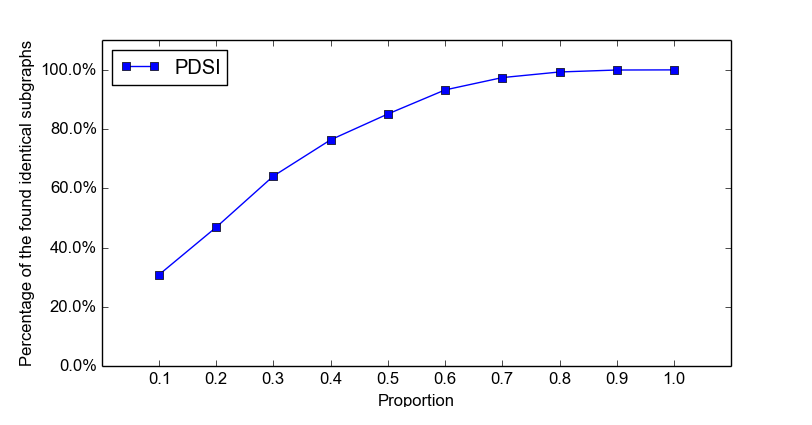
\includegraphics[width=\textwidth]{foundproportion-PPs.png}
    \caption{Percentage of the found identical subgraphs by PDSI with different proportions}
    \label{fig:foundproportion-PP}
  \end{center}
\end{figure}

\section{Evaluation of the Communication Costs for Synchronization}
\label{sec: evaluation-heterogeneity}

In the really world, the communication costs for synchronization are often heterogeneous. Therefore, we evaluate the vertex synchronization costs of the optimized DSI and geospatial simulation. Figure~\ref{fig:heterogeneity-ODSI} shows the number of vertices against the vertex synchronization costs in optimized DSI. The most vertices have the vertex synchronization costs below 200 kilobytes, while a few vertices have much more communication.

\begin{figure}[H]
  \begin{center}
    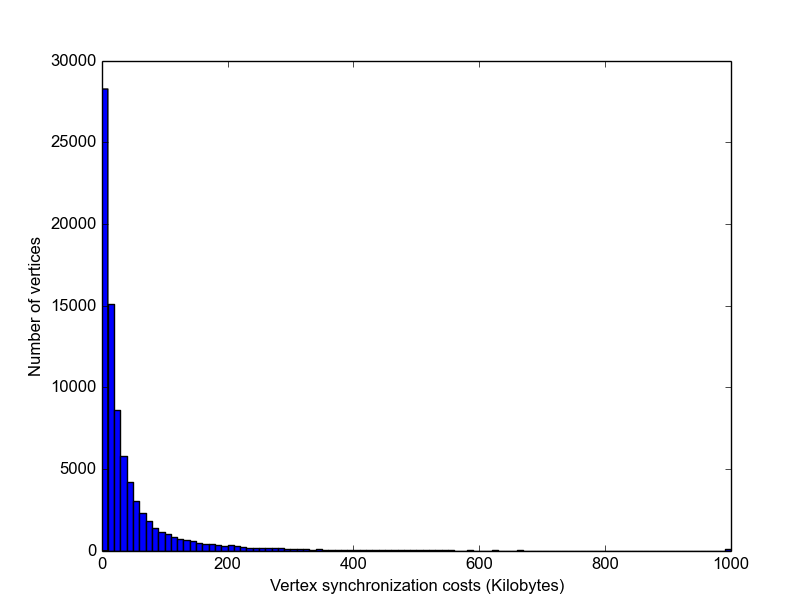
\includegraphics[width=\textwidth]{heterogeneity-ODSI.png}
    \caption{Vertex synchronization costs of optimized DSI on ego-Twitter graph with a 3-vertices pattern}
    \label{fig:heterogeneity-ODSI}
  \end{center}
\end{figure}

To evaluate geospatial simulation, we used the GPS trajectory dataset collected in Geolife project\footnote{http://research.microsoft.com/en-us/projects/geolife/default.aspx}. These trajectories were recorded by different GPS devices, and have a variety of sampling rates. Over 90\% of the trajectories were logged in a dense representation, e.g. every 1-5 seconds or every 5-10 meters per point. Although this dataset is wildly distributed in many cities, a subset of the data is used to simulate the agents mobility within Beijing, which contains in total 98 agents. The movements of agents are simulated in the time span of one day. The simulation time interval is 10 seconds. The area is divided into 10000 grids, each of which connects to its Moore neighborhood. Figure~\ref{fig:heterogeneity-ABCA} shows that the most vertices have very low communication costs for synchronization. This is mainly because that there are some hotspots in which the agents move.

\begin{figure}[H]
  \begin{center}
    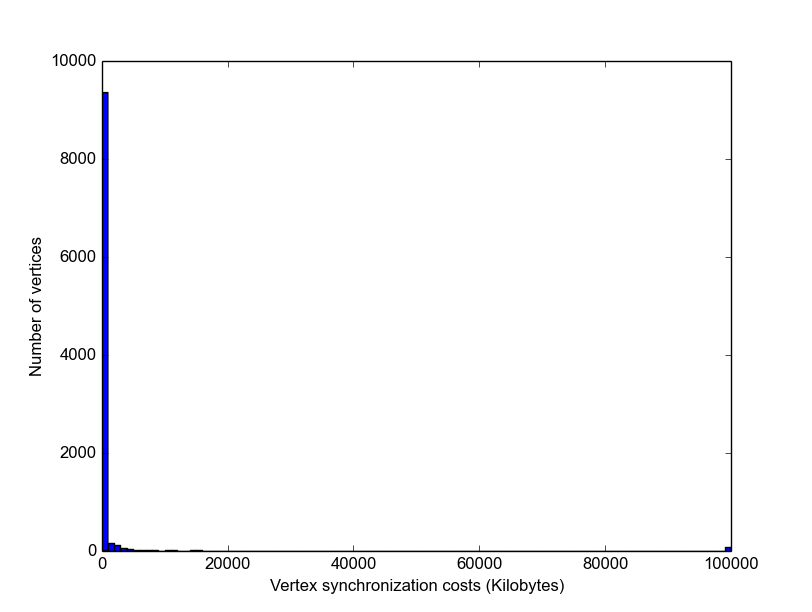
\includegraphics[width=\textwidth]{heterogeneity-ABCA.png}
    \caption{Vertex synchronization costs of geospatial simulation}
    \label{fig:heterogeneity-ABCA}
  \end{center}
\end{figure}


\section{Evaluation on GrapH}

GrapH is a framework prototype under developing in the University of Stuttgart, which takes the vertex synchronization costs into account to optimize graph partitioning. It loads graph by a static edge mapping algorithm and uses an adaptive partitioning strategy to migrate edges dynamically. 
%User can specify a parameter to control how many supersteps the adaptive partitioning to be performed, which lets user to balance the migration overhead in time.\textbf{TODO} 
Another feature of GrapH is that it keeps the graph in memory so that it can continuously perform different computation on the same graph with loading the graph only once. We evaluate the optimized DSI and geospatial simulation on GrapH to study the communication improvement by GrapH.

We performed optimized DSI on the ego-Twitter graph. We continuously executed 30 simple pattern queries, each of which consists of 2 or 3 vertices. We compare two executions with and without adaptive partitioning based on the PowerGraph pre-partitioned graph. The Figure~\ref{fig:si-pre-n10} shows that the accumulative communication including the migration costs between machines is reduced more than 20\% when using adaptive partitioning. As optimized DSI has complex computation and large data size, the costs for migrating edges are relatively low and negligible.

\begin{figure}[H]
  \begin{center}
    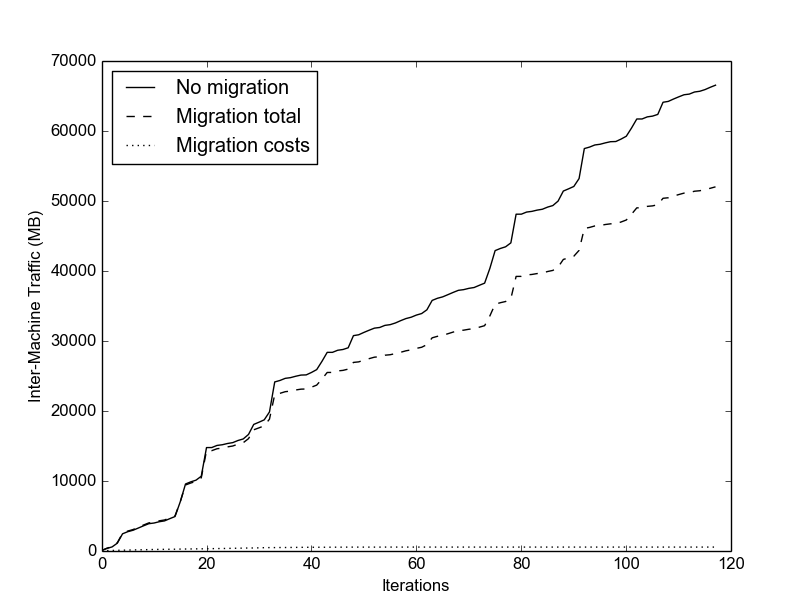
\includegraphics[width=\textwidth]{si-pre-n10.png}
    \caption{Accumulative inter-machine traffic of optimized DSI}
    \label{fig:si-pre-n10}
  \end{center}
\end{figure}

Figure~\ref{fig:si-pre-n10-c} shows the inter-machine traffic of each superstep. With the migration, the current inter-machine traffic is reduced gradually, and at the end the current traffic has been reduced about 30\%.

\begin{figure}[H]
  \begin{center}
    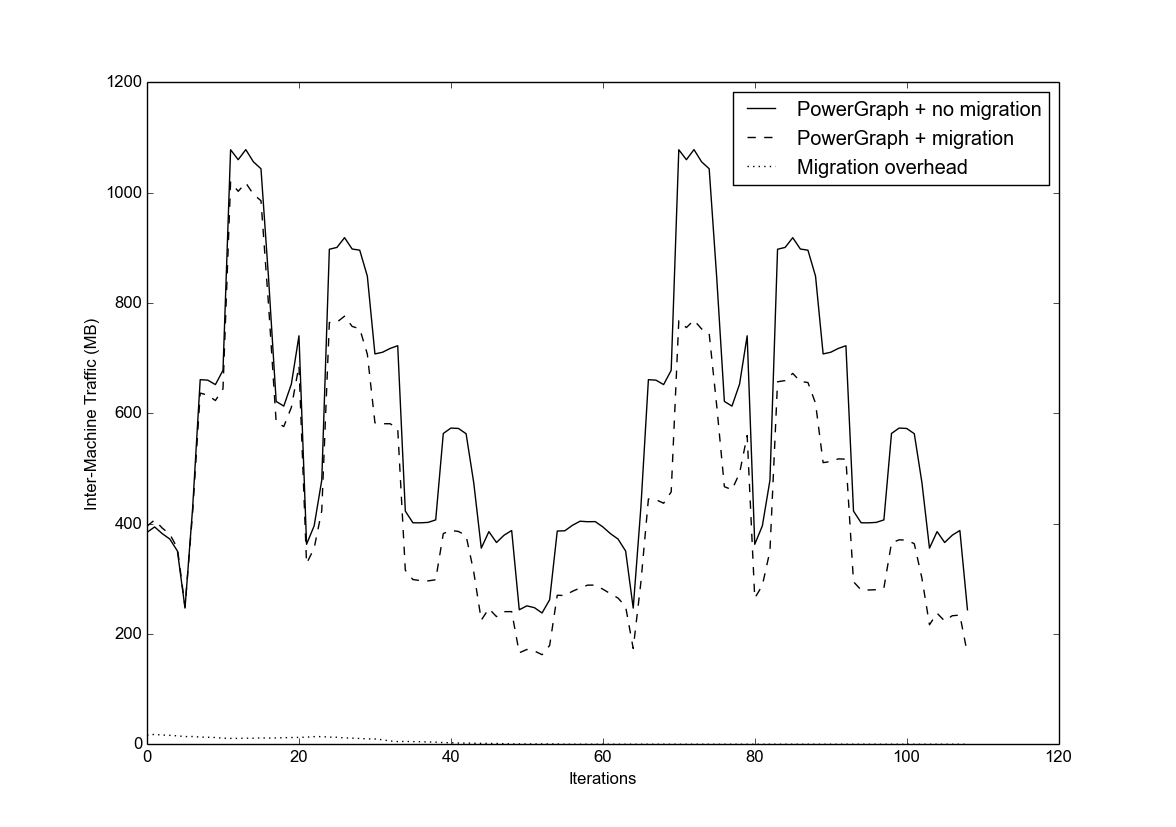
\includegraphics[width=\textwidth]{si-pre-n10-c.png}
    \caption{Current inter-machine traffic of optimized DSI}
    \label{fig:si-pre-n10-c}
  \end{center}
\end{figure}

In the evaluation of optimized DSI on GrapH, the adaptive partitioning strategy increases the latency slightly, which takes 5109 seconds, compared with 4904 seconds of the execution without adaptive partitioning.

We also performed the geospatial simulation with the same setting as we did in \ref{sec: evaluation-heterogeneity} except that the time interval is 1200 seconds. The PowerGraph pre-partitioned graph was loaded to GrapH and executed with and without adaptive partitioning. The latency is also increased by adaptive partitioning, which is 927 seconds, compared with 664 seconds of the execution without adaptive partitioning. The Figure~\ref{fig:ca-pre-n10} shows that the accumulative communication including the migration costs between machines is reduced more than 20\% by the adaptive repartition.

\begin{figure}[H]
  \begin{center}
    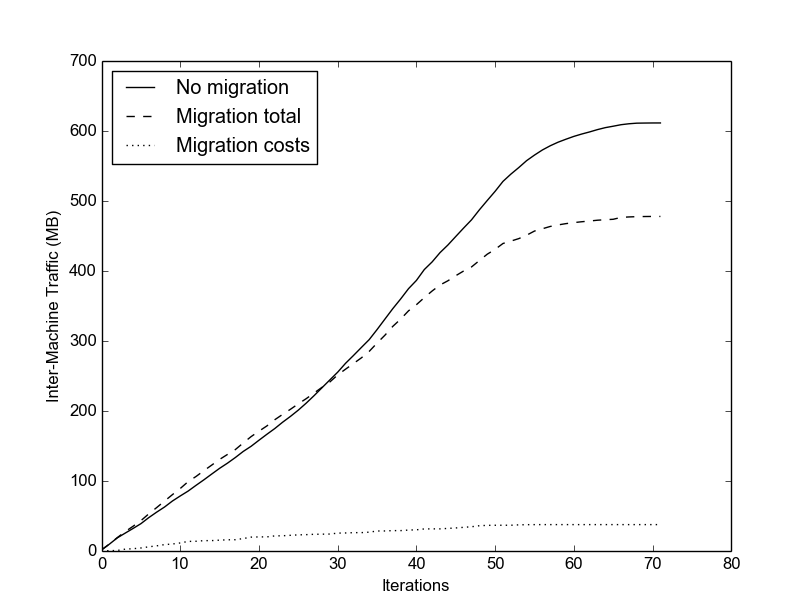
\includegraphics[width=\textwidth]{ca-pre-n10.png}
    \caption{Accumulative inter-machine traffic of geospatial simulation}
    \label{fig:ca-pre-n10}
  \end{center}
\end{figure}

Figure~\ref{fig:si-pre-n10-c} shows the inter-machine traffic of each superstep. At the beginning of migration, the current inter-machine traffic of the one with adaptive partitioning is a little bit higher than the one without adaptive partitioning due to the migration costs. However, the current inter-machine traffic has been reduced by the migration about 50\% at the end.

\begin{figure}[H]
  \begin{center}
    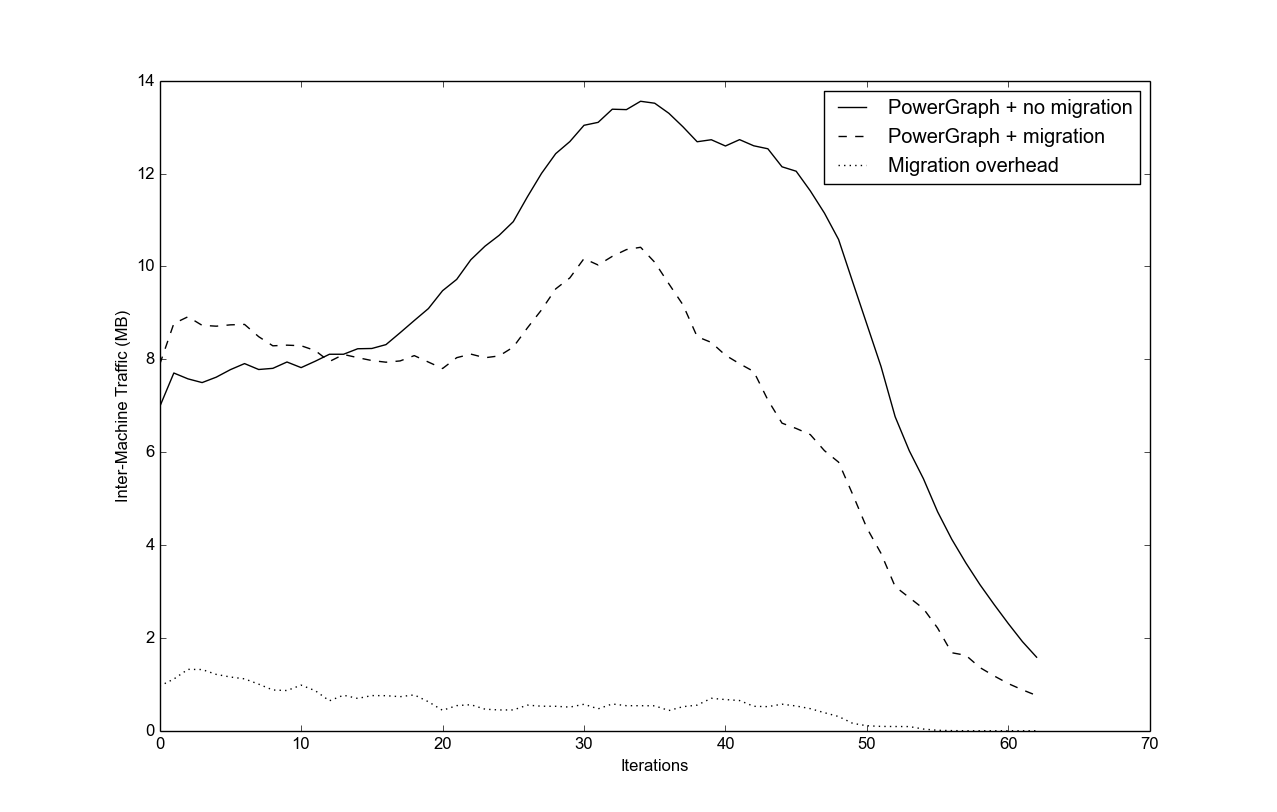
\includegraphics[width=\textwidth]{ca-pre-n10-c.png}
    \caption{Current inter-machine traffic of geospatial simulation}
    \label{fig:ca-pre-n10-c}
  \end{center}
\end{figure}